Following the training of DGCNN models on the BNCI 2014-001 Motor Imagery dataset, we present model performance, our analysis of the resulting graph structures, and internal representations. 
Rather than focusing on classification accuracy, our primary aim is to investigate the structural patterns and representational consistency that emerge across models trained with different seeds and hidden channel configurations.
\\
To assess the structural properties of the learned graphs, we compute a range of centrality metrics-including barycentres, Laplacian centrality, betweenness centrality, and current-flow betweenness centrality. These metrics allow us to identify nodes that frequently emerge as central or influential across training runs, providing insight into potential functional hubs in the EEG signal graph.
\\
In addition to structural analysis, we use CKA to quantify the similarity between internal representations learned by different models. CKA offers a robust measure for comparing the representations across layers and model instances, helping us understand the degree to which different DGCNNs converge on similar solutions despite differing initial conditions.

\subsection{Model Performance}
In total, we trained 756 GNNs across 84 random seeds and 9 different values for the number of hidden channels. These models achieved an average test accuracy of $48.9 \pm 1.2\%$, significantly outperforming the random-chance baseline of $25\%$. While model performance is not the central focus of this study, these results confirm that the networks have learned meaningful representations from the data, justifying further analysis of their internal graph structures and learned features.

\subsection{Graph Representations}
To visualize the structure of the graphs generated by the trained models, we present a representative example in Figure \ref{fig:Graphs}. This graph was produced by a model trained with seed 25243 and 24 hidden channels. While no two graphs are identical, this example illustrates the typical structure observed in our models. In the figure, red lines indicate strong edges with weights above 0.7, and the purple node marks the barycentre.
%Graphs
\begin{figure}[h!]
    \centering
    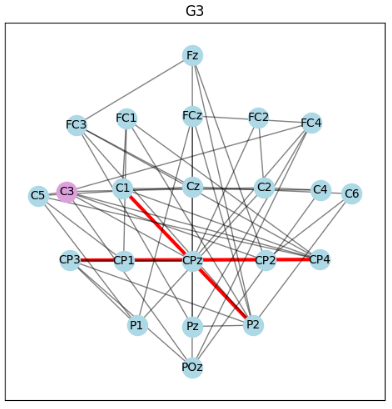
\includegraphics[width=0.45\linewidth]{img/single_graph1.png}
    \caption{Graph created by seed 25243 with 24 hidden channels; The purple node "C3" is highlighted as it is the identified barycentre of the graph; The red edges are the ones, considered strongest connections}
    \label{fig:Graphs}
\end{figure}

%CKA
\subsection{Average CKA}
Figure \ref{fig:CKA} presents the average CKA similarity across layers for all model pairs from the first 10 seeds. 
The diagonal of the matrix shows high similarity across corresponding layers, with the top three layers showing similarity scores above 0.9. 
The final two layers also exhibit strong consistency, with average similarity scores of 0.8 and 0.76, respectively.

\begin{figure}[h!]
    \centering
    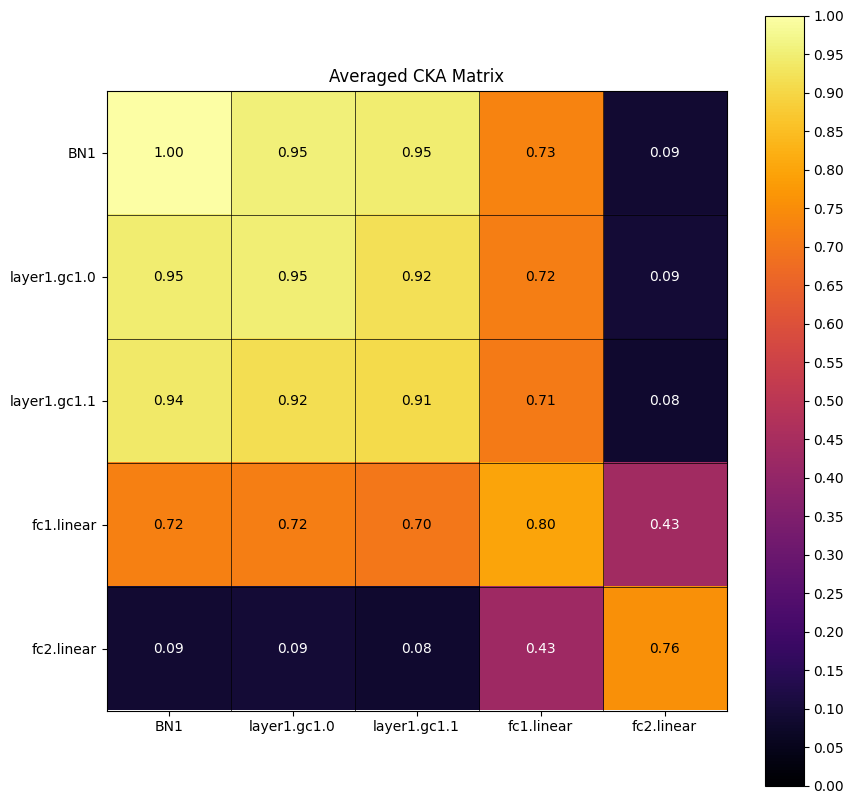
\includegraphics[width=0.7\linewidth]{img/CKA_10seeds.png}
    \caption{Average CKA for between the 90 models in the first 10 seeds}
    \label{fig:CKA}
\end{figure}

%Barycentres - histograms 
\subsection{Barycentre Bar Charts}
For each learned graph representation, we kept track of the barycentre nodes. We then made a bar chart of the barycentre frequency for all the models' learned graphs (Figure \ref{fig:barybar}).\\
From the plot, we can clearly see that C3,  CP3 and CP4 are more commonly the barycentre than all of the other nodes.
We also looked at the barycentre bar chart for the untrained models with the same seeds and parameters (Figure \ref{fig:barybar}) , to confirm that a difference occurs during training. For the untrained models, the barycentre counts are very similar for all the electrodes, as opposed to the trained model barycentre counts, in which we can clearly see that C3,  CP3 and CP4 are more frequent.
\vspace{0.5em}\\
To validate whether the difference between the barycentre counts of the trained and untrained models is statistically significant, we performed a Chi squared goodness of fit test. We obtain a $\chi^2$ test statistic of 212, which is higher than the critical value for significance level $\alpha=0.01$ and $K-1 = 21$ degrees of freedom, since we have 22 different electrodes. We thus reject the null hypothesis at a 1\% significance level, concluding that there is a significant difference in the barycentre counts before and after training the models.
\vspace{0.5em}\\
Furthermore, we compared the barycentre counts of the trained models' learned graph representations against the expected values of said counts under a uniform distribution. We have thus performed another Chi squared test to ensure there is a significant difference in the electrodes' probabilities of being barycentres. We obtain a $\chi^2$ test statistic of 172, which exceeds the critical value for significance level $\alpha=0.01$ with 21 degrees of freedom. We therefore reject the null hypothesis at the 1\% significance level, concluding that the electrodes don't have equal probabilities of being barycentres.
\begin{figure}[H]
    \centering
    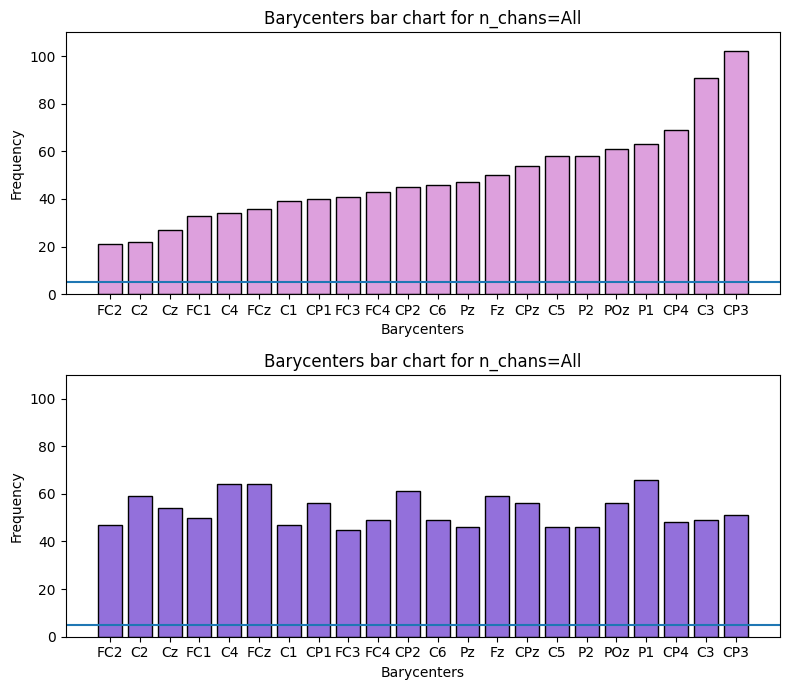
\includegraphics[width=0.8\linewidth]{img/barybar.png}
    \caption{Barycentres bar charts for the trained (top) and untrained (bottom) models; Order of untrained bars is based on the sorted ascending order of the trained results for comparison's sake; The blue line at the frequency of 5 marks the minimal frequency requirement for the execution of a $\chi^2$ test} 
    \label{fig:barybar}
\end{figure}
\noindent Since the ordering of nodes in the bar chart is arbitrarily chosen, a more meaningful way to visualise node-level results is by using the MNE library to generate a topomap,a heat map of electrode activity projected onto a head model, as shown in Figure~\ref{fig:bary_topo} (\cite{MNESoftware}, \cite{canonicalEEGjournal}). In the figure, we see the same information as in Figure~\ref{fig:barybar}, but now contextualised on the head. The deep red region on the lower left corresponds to the CP3 and C3 electrodes, indicating a high frequency of barycentre occurrences at that location.
\begin{figure}[H]
    \centering
    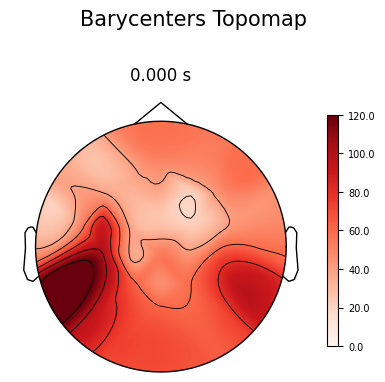
\includegraphics[width=0.5\linewidth]{img/bary_topo.png}
    \caption{Topological heat map showing barycentre node frequencies. Deeper red equals more centre occurrences}
    \label{fig:bary_topo}
\end{figure}
%Other centrality centres 
\noindent The bar charts for betweenness, current flow and Laplacian centre look similar, with C3,  CP3 and CP4 as the highest observed frequencies.
%Likelihood
\subsection{The Likelihood for Node Barycentres}
To quantify the significance of barycentre selection, we compute the likelihood of all nodes being selected as barycentres across all models.
\vspace{0.5em}\\
Table \ref{tab:likelihood} shows both types of likelihood we compute: the total likelihood (frequency) and the likelihood of a node being the centre, relative to a uniform distribution. It shows the two most frequently observed barycentres, C3 and CP3. We have showcased the two most likely nodes to occur across all centrality measures; the other 40 likelihoods can be found in  Appendix \ref{APP:Likelihood}
\vspace{0.5em}\\
We observe a clear distinction between trained and untrained models: in the trained models, C3 and CP3 are selected as barycentres in approximately $9$\% of cases, which is ~$90$\% more than the uniform.
In contrast, the untrained models show no strong preference, with frequencies near $4.5$\% and low differences from uniform expectations.
\vspace{0.5em}\\
These findings suggest that model training leads to the emergence of consistent structural patterns in the learned graph, particularly emphasising the C3 and CP3 electrodes, which are disproportionally selected as barycentres relative to a uniform distribution.
\begin{table}[H]
    \begin{subtable}[t]{0.45\textwidth}
        \centering
        \begin{tabular}{| l | c c |}
            \hline
            \textbf{Likelihood:} & \textbf{Total} & \textbf{Above}   \\       \textbf{C3}         &                &  \textbf{Uniform}\\ 
            \hline
            Trained & 8.77\% & 92.94\%  \\  
            Untrained & 4.74\% & 4.28\%  \\
            \hline
        \end{tabular}    
        \caption{C3 Likelihood}
    \end{subtable}
    \hfill
    \begin{subtable}[t]{0.45\textwidth}
        \centering
        \begin{tabular}{| l | c c |}
            \hline
            \textbf{Likelihood:} & \textbf{Total} & \textbf{Above}   \\       \textbf{CP3}         &                &  \textbf{Uniform}\\ 
            \hline
            Trained & 8.97\% & 92.34\%  \\  
            Untrained & 4.64\% & 2.08\% \\
            \hline
        \end{tabular}
        \caption{CP3 Likelihood}
    \end{subtable}
    \caption{The Likelihood of selecting C3 or CP3 as the barycentre, showing total frequency and the likelihood exceeding a uniform distribution.}
    \label{tab:likelihood}
\end{table}